\documentclass[11pt]{article}
\usepackage[margin=2.2cm]{geometry}
\usepackage{amsmath,amssymb,booktabs,tikz}
\usetikzlibrary{arrows.meta}
\newcommand{\II}{\mathrm{II}}
\title{Numerical evaluation of the three-loop $V\to q\bar q g$ finite remainders in full colour,\\
in decay and production kinematics}
\date{}
\begin{document}
\maketitle

\noindent All the full-colour finite remainders are linear combinations, with rational coefficients, of a finite set of
pure functions: iterated integrals over a 20-letter alphabet. Evaluating the remainders therefore means evaluating
this set of iterated integrals, in the decay region and in the production regions. These notes describe how:
\begin{itemize}
\item \textbf{Part 1:} the iterated integrals and their numerical evaluation in the decay region;
\item \textbf{Part 2:} the analytic continuation to the production regions;
\item \textbf{Part 3:} the assembly of the helicity amplitudes, and the spurious thresholds;
\item \textbf{Part 4:} the checks, and the precision on the LHC phase space.
\end{itemize}
The implementation is in \texttt{iter int /generators\_deq} (evaluator) and \texttt{package/} (the shippable package
\texttt{zgqq\_eval}).

%=====================================================================================================================
\part*{Part 1. The iterated integrals and their evaluation}

\section{Input}
\begin{itemize}
\item \textbf{Variables.} $x=s_{12}/q^2$, $y=s_{13}/q^2$, $z=s_{23}/q^2=1-x-y$. The decay region is the triangle
  $x,y,z>0$.
\item \textbf{Alphabet.} The letters are, with $r=\sqrt{xyz}$:
\[
\begin{array}{llll}
W_1=x, & W_2=y, & W_3=z, & W_4=1-x,\\
W_5=1-y, & W_6=x+y, & W_7=\dfrac{xz-ir}{xz+ir}, & W_8=\dfrac{xy-ir}{xy+ir},\\[2mm]
W_9=1-y-xy, & W_{10}=1-x-xy, & W_{11}=x-y+y^2, & W_{12}=y-x+x^2,\\
W_{13}=(1-x)^2-y, & W_{14}=(x+y)^2-y, & W_{15}=(x+y)^2-x, & W_{16}=(1-y)^2-x,\\
W_{17}=x+xy+y^2, & W_{18}=x^2+y+xy, & W_{19}=(1-y)^2+xy, & W_{20}=(1-x)^2+xy.
\end{array}
\]
  In the decay region the functions involve only $W_1$--$W_8$ and $W_{11}$--$W_{16}$; the others enter in the
  production regions (part 2). $W_7,W_8$ are the odd letters: they contain the square root $r$.
\item \textbf{The generators $G_k$.} The 579 functions $G_k$ of \texttt{Zgqq\_finite\_remainders/Generators.wl},
  in terms of which all the remainders are written. Each is a combination with rational coefficients of iterated
  integrals
  \[
    \II[a_1,\dots,a_n],\qquad d\,\II[a_1,\dots,a_n]=d\log W_{a_n}\;\II[a_1,\dots,a_{n-1}],
  \]
  of weight $n\le6$. By weight there are $1,5,24,75,203,247,24$ of them.
\end{itemize}

\section{Boundary conditions}
The base point is the corner $c_1=(x,y)=(0,0)$, with shuffle regularisation: $\II[\,]=1$ and every non-empty iterated
integral vanishes at the base point once its logarithmic divergences are regularised. Near the corner each function is
a polynomial in $\log x$, $\log y$ times power series, and the regularised constants are zero. All boundary
information is therefore exact. Its values at the other two corners $c_2=(1,0)$ and $c_3=(0,1)$ follow by exact
transport along the edges (GPLs).

\section{The differential equation}
\paragraph{Word space.} A function of weight $n$ is a combination of words with rational coefficients,
$f=\sum_{\mathbf a}c_{\mathbf a}\,\II[\mathbf a]$, $\mathbf a=(a_1,\dots,a_n)$. The \emph{word space} of weight $n$ is the
vector space with one basis vector for each word $\mathbf a$. The function $f$ is identified with its vector of
coefficients $(c_{\mathbf a})$ there.
\begin{itemize}
\item \textbf{Why this is allowed.} The $d\log W_i$ are linearly independent, so iterated integrals with different
  words are linearly independent functions. A linear relation between functions is therefore the same as a linear
  relation between their coefficient vectors. Questions such as ``is this function a combination of those?'' become
  exact linear algebra on rational vectors.
\item \textbf{Size.} Only the words that actually occur matter: 1872 of the $20^5=3.2\cdot10^6$ possible words at
  weight 5, and 9356 of $6.4\cdot10^7$ at weight 6.
\end{itemize}

\paragraph{Example.} With $W_1=x$, $W_2=y$, $W_3=z$, the weight-2 function
\[
  f=\II[1,2]+2\,\II[2,1]-\II[1,3]
\]
is the vector with entries $1$, $2$, $-1$ on the words $(1,2)$, $(2,1)$, $(1,3)$, and 0 on all others. Since
$d\,\II[a_1,a_2]=d\log W_{a_2}\,\II[a_1]$,
\[
  df=d\log y\;\II[1]+2\,d\log x\;\II[2]-d\log z\;\II[1] .
\]
The coefficient of each $d\log W_i$ is a function of weight 1: here $S_2f=\II[1]$, $S_1f=2\,\II[2]$ and
$S_3f=-\II[1]$. These are the strips defined below.

\paragraph{Differentiation.} Each iterated integral is differentiated through its last letter, so collecting the terms
of $df$ by the last letter gives
\[
  df=\sum_{i=1}^{20}d\log W_i\;S_if,\qquad S_if=\sum_{\mathbf a'}c_{(\mathbf a',i)}\,\II[\mathbf a'] .
\]
In words, $S_if$ keeps the words of $f$ that end in the letter $i$ and deletes that last letter. It is a function of
weight $n-1$, the coefficient of $d\log W_i$ in $df$; we call it the \emph{strip} of $f$ along $i$. In word space $S_i$
is a matrix with entries 0 and 1, which sends the word $(\mathbf a',i)$ to $\mathbf a'$ and every other word to zero.

\paragraph{Closure: the total generators $g_k$.} To integrate the $G_k$ we need every function that appears in their
derivatives, and in the derivatives of those, down to weight 0. So we define, from the top down,
\begin{gather*}
  V_6=\operatorname{span}\{G_k\text{ of weight 6}\},\\
  V_n=\operatorname{span}\{G_k\text{ of weight }n\}+\operatorname{span}\{S_if:\ f\in V_{n+1},\ i=1,\dots,20\}
  \qquad(n=5,\dots,1),
\end{gather*}
and $V_0=\{\text{constants}\}$. By construction $S_i$ maps $V_n$ into $V_{n-1}$, so the spaces are closed under
differentiation. The \emph{total generators} $g_k$, $k=1,\dots,503$, are a basis of these spaces: a maximal set of
linearly independent functions among the $G_k$ and the strips, with the $G_k$ taken first.
\begin{center}
\begin{tabular}{lccccccc|c}\toprule
weight $n$ & 0 & 1 & 2 & 3 & 4 & 5 & 6 & total \\ \midrule
generators $G_k$ & 1 & 5 & 24 & 75 & 203 & 247 & 24 & 579 \\
independent $G_k$ & 1 & 5 & 24 & 75 & 113 & 245 & 24 & 487 \\
new functions from the strips & & & & & & 16 & & 16 \\
total generators $g_k$: $\dim V_n$ & 1 & 5 & 24 & 75 & 113 & 261 & 24 & 503 \\ \bottomrule
\end{tabular}
\end{center}
\begin{itemize}
\item \textbf{Dependent generators.} The $G_k$ are not linearly independent over $\mathbb Q$. Only 487 of the 579
  are; at weight 4, for instance, the 203 generators span 113 dimensions.
\item \textbf{The independent $G_k$ alone are not closed.} The strips of the weight-6 generators contain 16 weight-5
  functions that are not combinations of any $G_k$. Without them the derivatives could not be expressed in terms of
  the unknowns.
\end{itemize}
So the system to integrate is that of the 503 total generators $g_k$. Each $G_k$ is a rational combination of the
$g_k$. The choice of basis of the spaces $V_n$ does not change the count, only the numerics (below). All of this is
exact linear algebra in word space, with rational coefficients.

\paragraph{The orthonormal system (double precision).} For each $n\le5$ we choose an orthonormal basis of $V_n$ in word
space, where two different words are orthonormal: a matrix $Q_n$ whose columns are coefficient vectors, with
$Q_n^TQ_n=1$. The unknowns are the corresponding
functions, the \emph{states}
\[
  \phi_n=Q_n^T\,\II_n\qquad(\II_n:\text{ the vector of the words of weight }n),
\]
479 of them for $n\le5$. They span the same spaces as the $g_k$ of weight $\le5$. The 24 weight-6 functions never
appear in any derivative (there is no weight 7), so they need no equation of their own: a single quadrature along the
path gives them (the read-off below). The derivatives of the states follow from the strips. $S_iQ_n$ lies in
$V_{n-1}$, the span of $Q_{n-1}$, so $S_iQ_n=Q_{n-1}\,(Q_{n-1}^TS_iQ_n)$, and
\[
  d\phi_n=\sum_id\log W_i\;A_i^{(n)}\,\phi_{n-1},\qquad A_i^{(n)}=(Q_{n-1}^TS_iQ_n)^T .
\]
Every entry satisfies $|A|\le1$: $S_i$ only moves words, and $Q$ has orthonormal columns. The generators are read off
along the integration from their own strips, $dG_k=\sum_id\log W_i\,\big(R_i^{(n)}\phi_{n-1}\big)_k$ for $G_k$ of weight
$n$, with $R_i^{(n)}$ the coefficients of $S_iG_k$ in the basis $Q_{n-1}$.

\paragraph{Example.} Let a weight-2 space be spanned by
\[
  f_1=\II[1,2]+\II[2,1],\qquad f_2=\II[1,2]-\II[2,1]+\II[1,3].
\]
\begin{itemize}
\item \textbf{The orthonormal basis.} On the words $(1,2),(2,1),(1,3)$ the coefficient vectors are $f_1=(1,1,0)$ and
  $f_2=(1,-1,1)$. They happen to be orthogonal already, so normalising them gives
  $Q_2=\big(\tfrac1{\sqrt2}(1,1,0),\ \tfrac1{\sqrt3}(1,-1,1)\big)$. In general $Q_n$ comes from a QR decomposition of the
  vectors of the $g_k$.
\item \textbf{The states and their equations.} The states are $\phi_{2,1}=f_1/\sqrt2$ and $\phi_{2,2}=f_2/\sqrt3$. At
  weight 1 the words are already orthonormal, so $\phi_1=(\II[1],\II[2],\dots)$. The strips give
  \[
    d\phi_{2,1}=\tfrac1{\sqrt2}\big(d\log y\;\II[1]+d\log x\;\II[2]\big),\qquad
    d\phi_{2,2}=\tfrac1{\sqrt3}\big(d\log y\;\II[1]-d\log x\;\II[2]+d\log z\;\II[1]\big),
  \]
  i.e.\ the matrices $A_i^{(2)}$ have entries $\pm1/\sqrt2$, $\pm1/\sqrt3$ and 0, all of size at most 1.
\item \textbf{A badly scaled basis for comparison.} The pair $f_1$, $f_2'=f_2+1000\,f_1$ spans the same space. But the
  equation of $f_2'$ has coefficients $\sim1000$. Recovering $f_2=f_2'-1000\,f_1$ from the unknowns cancels two terms
  of size $\sim1000$, so three digits are lost; the integration errors are amplified the same way. With the $g_k$ of the real system such effects reach many orders of
  magnitude. The orthonormal basis avoids them by construction.
\end{itemize}

\paragraph{The integer system (exact, quad precision).} For exact work we use a basis over the integers of the same
spaces (HNF and LLL), in which every connection matrix $M_i$ is integer:
\[
  dF=\sum_i d\log W_i\;M_iF .
\]
At weights $0$--$4$ and $6$ it is a true integral basis with the same counts. At weight 5 a true integral basis needs
huge integers, so we keep a redundant spanning set instead: the 247 generators and 97 strips of the weight-6
generators, 344 functions for 261 dimensions. That makes 586 functions in total, and the entries are at most
$3.5\cdot10^5$. The $G_k$ are integer combinations of the 586 functions $F$, and the states $\phi_n$ are exact rational
combinations of them, so values carry over exactly between the two systems.

\paragraph{Why the orthonormal system.}
\begin{itemize}
\item \textbf{A basis is needed.} The generators are linearly dependent, so they cannot be integrated directly as a
  system: the unknowns must be a basis of the spaces $V_n$, e.g.\ the total generators $g_k$.
\item \textbf{A naive basis is badly conditioned.} The natural choice of unknowns, the $g_k$ themselves, gives
  connection matrices with rational entries of about 100 digits. The integer basis brings them down to integers, but
  still up to $3.5\cdot10^5$, while its functions reach $4.5\cdot10^4$. The derivatives are then sums of large terms that
  cancel, so every step of the integration loses digits.
\item \textbf{The orthonormal basis is well conditioned.} With $Q_n$ orthonormal in word space, $A=Q^TSQ$ has all
  entries $|A|\le1$, since $S$ only moves words, and the states $\phi_n$ stay of order one ($|\phi|\le3$ at $P_0$). In double
  precision this gives the best accuracy: at the same points the median error is $2\cdot10^{-12}$, against
  $10^{-11}$ for the integer system integrated in double. It also uses the minimal number of functions: 479 states plus
  the 24 weight-6 read-offs.
\item \textbf{The price.} $Q_n$ comes from a floating-point orthonormalisation, so the matrices $A$ are exact only to
  double precision. This system cannot go beyond double, and its matrix rounding is the systematic error discussed in
  section~\ref{sec:prec}. For quad precision and for the exact series we use the integer system.
\end{itemize}

\section{The reference point $P_0$ of the decay triangle}
All evaluations start from one reference point at the centre of the triangle, $P_0=(0.3,0.3)$, where the 586 functions
are stored once and for all. They are determined to high precision as follows.

\paragraph{1. A double series at the corner.} From the exact series of the blow-up charts at $c_1$, chart 1 ($x=ty^2$)
and its mirror ($y=tx^2$), each to order $t^{16}$, $B^{48}$, we undo the blow-up ($t=x/y^2$,
$\log t=\log x-2\log y$). The result is a genuine double series,
\[
  F(x,y)=\sum c\;x^{a/2}\,y^{b/2}\,\log^kx\,\log^ly,\qquad c\text{ exact rational (times 1 or }i).
\]
No negative powers appear, and the two charts agree exactly on all $1.3\cdot10^6$ terms they share. Several letters
vanish at $c_1$ ($x+y$, $x-y+y^2$, $(x+y)^2-x$, \dots), but the functions do not see them there. The union of the two
charts holds every term of total degree $\frac{a+b}2\le32$, so the truncation error is $\approx(|x|+|y|)^{33}$.

\paragraph{2. Two start points,} $S_A=(0.05,0.05)$ and $S_B=(0.04,0.06)$, evaluated from the series at 40 digits
(truncation $10^{-34}$).

\paragraph{3. Quad transport over two paths.} From each start point we integrate the integer system to $P_0$ along its
own complex-deformed straight path:
\[
  x(t)=S_x+\big(t+4i\,\delta_x\,t(1-t)\big)(0.3-S_x),\qquad y(t)=S_y+\big(t+4i\,\delta_y\,t(1-t)\big)(0.3-S_y),
\]
with $\delta_A=(-0.15,-0.25)$ (below the real plane) and $\delta_B=(0.1,0.2)$ (above). The root $r$ is integrated
along ($dr=r\,d\log(xyz)/2$).
\begin{itemize}
\item The integrator is Bulirsch--Stoer (modified midpoint, polynomial extrapolation) in double-double arithmetic
  ($\approx32$ digits), with tolerance $10^{-32}$ relative to the largest function.
\item Two points matter. Each half of a double-double number must be read back as a double. And the extrapolation
  weights $m_l^2/(m_j^2-m_l^2)$ ($m_j$ the numbers of substeps) must be exact in double-double; in double they cap the accuracy at $10^{-24}$.
\end{itemize}

\paragraph{Result.} The two determinations agree to $3\cdot10^{-28}$ relative to the largest function
($4.5\cdot10^4$): 27--28 digits. Further start points ($(0.06,0.06)$, $(0.06,0.04)$, $(0.08,0.08)$) and a second path
from $S_A$ agree within $2\cdot10^{-27}$. The values are mapped exactly onto the states $\phi_n$ of the double system.

\begin{center}
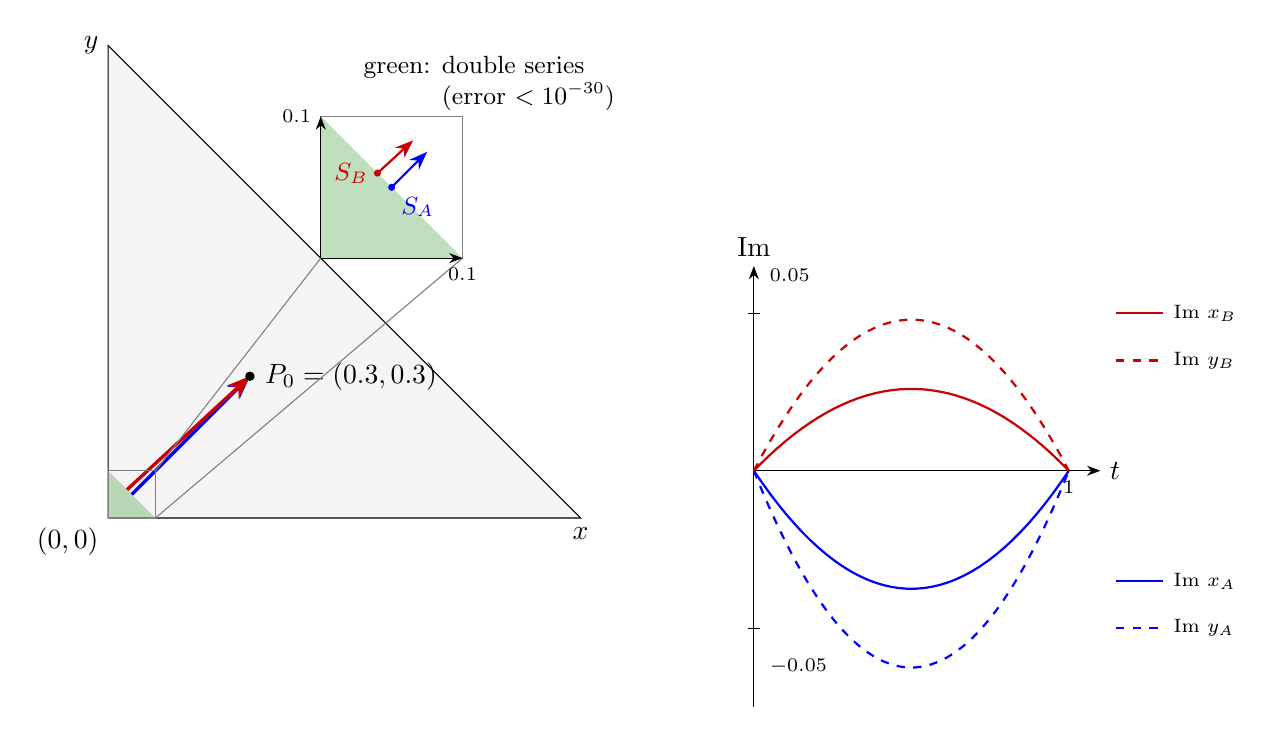
\begin{tikzpicture}[>=Stealth]
  \begin{scope}[scale=6]
    \fill[gray!8] (0,0)--(1,0)--(0,1)--cycle; \draw (0,0)--(1,0)--(0,1)--cycle;
    \node[below left] at (0,0) {$(0,0)$}; \node[below] at (1,0) {$x$}; \node[left] at (0,1) {$y$};
    \fill[green!50!black,opacity=0.25] (0,0)--(0.1,0)--(0,0.1)--cycle;
    \draw[very thick,blue,->] (0.05,0.05)--(0.3,0.3);
    \draw[very thick,red!80!black,->] (0.04,0.06)--(0.3,0.3);
    \fill (0.3,0.3) circle (0.01) node[right=2pt] {$P_0=(0.3,0.3)$};
    \draw[gray] (0,0) rectangle (0.1,0.1); \draw[gray] (0.1,0.1)--(0.45,0.55); \draw[gray] (0.1,0)--(0.75,0.55);
    \node[font=\small,align=left,anchor=west] at (0.52,0.92) {green: double series\\ \phantom{green: }(error $<10^{-30}$)};
  \end{scope}
  \begin{scope}[shift={(2.7,3.3)},scale=18]
    \fill[white] (0,0) rectangle (0.1,0.1); \draw[gray] (0,0) rectangle (0.1,0.1);
    \fill[green!50!black,opacity=0.25] (0,0)--(0.1,0)--(0,0.1)--cycle;
    \draw[->] (0,0)--(0.1,0); \draw[->] (0,0)--(0,0.1);
    \draw[blue,thick,->] (0.05,0.05)--(0.075,0.075); \draw[red!80!black,thick,->] (0.04,0.06)--(0.0652,0.0831);
    \fill[blue] (0.05,0.05) circle (0.0025) node[below right,font=\small] {$S_A$};
    \fill[red!80!black] (0.04,0.06) circle (0.0025) node[left,font=\small] {$S_B$};
    \node[font=\scriptsize,below] at (0.1,0) {$0.1$}; \node[font=\scriptsize,left] at (0,0.1) {$0.1$};
  \end{scope}
  \begin{scope}[shift={(8.2,0.6)},xscale=4,yscale=40]
    \draw[->] (0,0)--(1.1,0) node[right] {$t$}; \draw[->] (0,-0.075)--(0,0.065) node[above] {Im};
    \node[font=\scriptsize,below] at (1,0) {1};
    \draw[blue,thick,domain=0:1,samples=40] plot (\x,{-0.15*\x*(1-\x)});
    \draw[blue,thick,dashed,domain=0:1,samples=40] plot (\x,{-0.25*\x*(1-\x)});
    \draw[red!80!black,thick,domain=0:1,samples=40] plot (\x,{0.104*\x*(1-\x)});
    \draw[red!80!black,thick,dashed,domain=0:1,samples=40] plot (\x,{0.192*\x*(1-\x)});
    \node[font=\scriptsize,anchor=west] at (0.02,0.062) {$0.05$}; \draw (-0.02,0.05)--(0.02,0.05);
    \node[font=\scriptsize,anchor=west] at (0.02,-0.062) {$-0.05$}; \draw (-0.02,-0.05)--(0.02,-0.05);
    \draw[red!80!black,thick] (1.15,0.05)--(1.3,0.05) node[right,font=\scriptsize,black] {Im $x_B$};
    \draw[red!80!black,thick,dashed] (1.15,0.035)--(1.3,0.035) node[right,font=\scriptsize,black] {Im $y_B$};
    \draw[blue,thick] (1.15,-0.035)--(1.3,-0.035) node[right,font=\scriptsize,black] {Im $x_A$};
    \draw[blue,thick,dashed] (1.15,-0.05)--(1.3,-0.05) node[right,font=\scriptsize,black] {Im $y_A$};
  \end{scope}
\end{tikzpicture}
\end{center}
\noindent Figure 1. The construction of $P_0$. Left: the two paths (real part) from the series region to $P_0$, with a
zoom of the corner. Right: the imaginary parts along the paths, $4\delta\,t(1-t)(0.3-S)$.

\section{Transport to any point}
A point $P$ of the triangle is reached from $P_0$ along a complex-deformed straight path,
$z(t)=P_0+\big(t+4i\delta\,t(1-t)\big)(P-P_0)$ for each coordinate.
\begin{itemize}
\item \textbf{The deformation.} The letters vanish on curves, and their complex zeros can lie on a straight path. Along
  the path every letter is a polynomial of degree $\le4$ in $t$, so its zeros are found as roots. We use the first
  deformation from a fixed list whose path keeps a distance $\ge10^{-3}$ (in $t$) from every zero.
\item \textbf{Double.} The orthonormal system is integrated by Bulirsch--Stoer (\texttt{cpp/tridents\_bs}). This takes
  about 0.07 s per point.
\item \textbf{Quad.} The integer system is integrated in double-double (\texttt{cpp/iter\_quad}), at 5--10 s per point.
\end{itemize}
The method works anywhere inside the triangle. Close to its edges, where the remainders approach their unresolved
(soft, collinear, high-energy) limits, double precision loses digits (section~\ref{sec:prec}). There, quad or the corner
series are the right tools.

\section{Assessing the precision}\label{sec:prec}
\paragraph{Where digits are lost.} The remainder is a large sum of rational functions times generators (part 3). Near
the edges the rational functions grow (like $1/x^3$, or $(x+y)^{-5}$ at the corners) while the generators grow only
logarithmically, so the terms cancel. The sum of $|$terms$|$ exceeds the value by $\sim10^4$ in the bulk and up to
$10^9$ near the edges. Double keeps $16-\log_{10}(\text{cancellation})$ digits; quad keeps 16 more.

\paragraph{Method 1: double against quad.} The same point is evaluated in double and in quad. The difference is the
actual error of double, since quad is good to $\sim10^{-23}$ in the bulk. This is the reference test, used for all
the precision statements below.

\paragraph{Method 2: double on two paths (the built-in estimate).} Every point is evaluated twice in double, on two
different deformed paths, and the estimate is
\[
  \varepsilon_{\rm est}=10\,|R_1-R_2|+\epsilon\sum|\text{terms}|,\qquad\epsilon=10^{-13}.
\]
The path difference catches the path-dependent integration error, but not what both paths share:
\begin{itemize}
\item \textbf{The start values.} With the old double-precision $P_0$, whose errors reached $5\cdot10^{-8}$ absolute,
  the estimate missed values in the subleading colour layers. The quad $P_0$ removed this.
\item \textbf{The systematic error of the double system.} Its matrices are floating point. The generator errors of
  the two paths are 85\% correlated, and changing the integration tolerance from $10^{-11}$ to $10^{-15}$ does not
  change them. Amplified by the cancellation, this is covered by the term $\epsilon\sum|\text{terms}|$.
\end{itemize}
Against method 1 the estimate was an upper bound in every test, but about 1000 times too large. A sharper option is
an independent second evaluation with the integer system in double: it bounds the error to $\sim40$ times, with
3 misses in 924.

%=====================================================================================================================
\part*{Part 2. Analytic continuation to the production regions}

\section{The new variables and the new triangle}
In a production region one invariant exceeds $q^2$ and the other two are negative. We take $z>1$ as the example; it is
the channel with partons 2 and 3 incoming. With
\[
  v=\frac1z,\qquad u=-\frac yz,\qquad w=-\frac xz=1-u-v,\qquad u,v,w>0,
\]
the region becomes a triangle again. $v=q^2/\hat s$ is the inverse energy: $v\to1$ is threshold and $v\to0$ is high
energy. In the code the region's triangle is written $(X,Y)=(w,u)$ with $Z=v$, so $(x,y)=(-X/Z,-Y/Z)$. The other regions
are analogous:
\[
  x>1:\ (x,y,z)=(1/Z,-X/Z,-Y/Z),\qquad y>1:\ (x,y,z)=(-X/Z,1/Z,-Y/Z).
\]

\section{The differential equation in the new variables}
Substituting the map into the twenty letters, every letter becomes a constant times a power of $Z$ times a letter of the
same alphabet in $(X,Y)$: \emph{the alphabet closes}. For $z>1$:
\begin{center}\small
\begin{tabular}{@{}cccccccccccc@{}}\toprule
$W_1$&$W_2$&$W_3$&$W_4$&$W_5$&$W_6$&$W_{11}$&$W_{12}$&$W_{13}$&$W_{14}$&$W_{15}$&$W_{16}$\\
$W_1'/Z$&$W_2'/Z$&$1/Z$&$W_5'/Z$&$W_4'/Z$&$W_6'/Z$&$W_{12}'/Z^2$&$W_{11}'/Z^2$&$W_9'/Z^2$&$W_{18}'/Z^2$&$W_{17}'/Z^2$&$W_{10}'/Z^2$\\\bottomrule
\end{tabular}
\end{center}
So $d\log W_i=\sum_jc_{ij}\,d\log W'_j$ with integer $c_{ij}$, and the region carries the same kind of system:
\[
  dF=\sum_jd\log W'_j\;M'_jF,\qquad M'_j=\sum_ic_{ij}M_i\quad(\text{and }A'^{(n)}_j=\sum_ic_{ij}A_i^{(n)}\text{ for the orthonormal system}).
\]
The same integrators apply unchanged. In the region the letters $W_9,W_{10},W_{17},W_{18}$ enter, but their zeros lie
outside the region's triangle.

\paragraph{The square root and its Galois symmetry.} The odd letters $W_{7,8}=(a-ir)/(a+ir)$ contain $r=\sqrt{xyz}$.
\begin{itemize}
\item \textbf{The symmetry.} Under the Galois conjugation $r\to-r$, $W_{7,8}\to1/W_{7,8}$, so their $d\log$ change sign.
  The functions split into even and odd parts, and the odd ones enter the remainders multiplied by $i/r$ (one of the
  transcendental multipliers). Each remainder is therefore invariant, provided the same branch of $r$ is used in the
  letters and in the prefactor.
\item \textbf{The continued branch.} In the region $xyz>0$ again, but the continuation fixes the branch. With
  $\log x\to\log|x|+i\pi$ and $\log y\to\log|y|+i\pi$ (next section), $\sqrt x\sqrt y\to(i\sqrt{|x|})(i\sqrt{|y|})$, so
  \[
    r\to-\sqrt{|xyz|}=-\frac{\sqrt{XYZ}}{Z^2}.
  \]
\item \textbf{In the region's variables.} Expressed through the region's own root $R=\sqrt{XYZ}$, the odd letters map
  to $d\log W_7\to d\log W_7'+d\log W_8'$ and $d\log W_8\to-d\log W_8'$. The rational prefactors are evaluated with
  $r=-\sqrt{|xyz|}$.
\end{itemize}

\section{The continued boundary values}
The corner $X,Y\to0$ of the region's triangle (threshold) is a decay corner approached from the other side: $c_1$ for
$z>1$, $c_2$ for $x>1$, $c_3$ for $y>1$. Its two small variables are $(-X/Z,-Y/Z)$, i.e.\ $(x,y)$ for $z>1$. Both cross
zero from above (Feynman prescription, every invariant $+i0$), so the corner series is continued by
\[
  \log s\to\log|s|+i\pi,\qquad \sqrt s\to i\sqrt{|s|}\qquad\text{for each small variable }s .
\]
In a blow-up chart $\text{SMALL}=t\,\text{BIG}^2$ this reads $\log t\to\log|t|-i\pi$, $\log B\to\log|B|+i\pi$.
\begin{itemize}
\item \textbf{$z>1$ (corner $c_1$).} The decay double series, evaluated at $x=-X/Z$, $y=-Y/Z$ with this continuation.
\item \textbf{$x>1$, $y>1$ (corners $c_2$, $c_3$).} Here the functions are \emph{not} double series in the two small
  variables, because the letter $1-x=y+z$ (resp.\ $1-y=x+z$) vanishes at the corner. Undoing the blow-up leaves
  negative powers already at weight 1, in about 520 functions. We use the exact series of one chart instead (chart
  $y=tz^2$ at $c_2$, $x=tz^2$ at $c_3$), continued as above. It is evaluated at small $|t|\approx0.02$, i.e.\ at start
  points close to the edge $X=0$.
\end{itemize}
The series coefficients are exact. In the decay, the chart series at $c_2$ and $c_3$ agree with a quad integration from
$P_0$ to $10^{-27}$, which checks their boundary constants.

\begin{center}
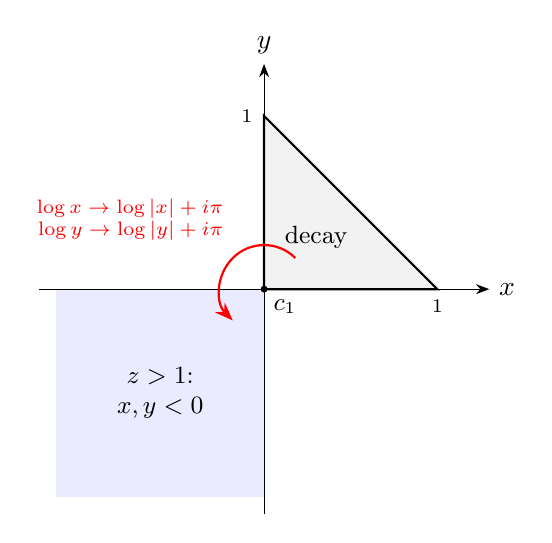
\begin{tikzpicture}[scale=2.2,>=Stealth]
  \fill[blue!8] (0,0)--(-1.2,0)--(-1.2,-1.2)--(0,-1.2)--cycle;
  \fill[gray!10] (0,0)--(1,0)--(0,1)--cycle; \draw[thick] (0,0)--(1,0)--(0,1)--cycle;
  \draw[->] (-1.3,0)--(1.3,0) node[right] {$x$}; \draw[->] (0,-1.3)--(0,1.3) node[above] {$y$};
  \node[font=\small] at (0.3,0.3) {decay};
  \node[align=center,font=\small] at (-0.6,-0.6) {$z>1$:\\ $x,y<0$};
  \node[font=\scriptsize] at (1,-0.1) {$1$}; \node[font=\scriptsize] at (-0.1,1) {$1$};
  \fill (0,0) circle (0.02); \node[font=\small] at (0.12,-0.1) {$c_1$};
  \draw[->,red,thick] (0.18,0.18) arc (45:225:0.255);
  \node[red,font=\scriptsize,align=right,anchor=east] at (-0.18,0.4) {$\log x\to\log|x|+i\pi$\\ $\log y\to\log|y|+i\pi$};
\end{tikzpicture}
\end{center}
\noindent Figure 2. The region $z>1$ is the quadrant $x,y<0$ of the plane $(x,y)$; in its own variables it is the
triangle $(X,Y)=(w,u)$. It touches the decay triangle at the corner $c_1$, which is the threshold corner $X,Y\to0$ of the
region. The continuation is the half-turn around $c_1$, with both small variables crossing zero from above.

\section{The reference point of each region}
Each region's $P_0$ is its hub $(X,Y)=(0.3,0.3)$, determined exactly as in the decay. We take two start points near the
region's corner, evaluated from the continued series, and transport each in quad along its own path, with the region's
integer system.
\begin{center}
\begin{tabular}{lllll}\toprule
region & corner, series & start points $(X,Y)$ & truncation & two paths agree \\ \midrule
$z>1$ & $c_1$, double series & $(0.05,0.05)$, $(0.04,0.06)$ & $10^{-33}$ & $1.5\cdot10^{-27}$ \\
$x>1$ & $c_2$, chart $y=tz^2$ & $(0.001,0.2)$, $(0.0005,0.15)$ & $2\cdot10^{-29}$ & $1.9\cdot10^{-27}$ \\
$y>1$ & $c_3$, chart $x=tz^2$ & $(0.001,0.2)$, $(0.0005,0.15)$ & $5\cdot10^{-30}$ & $2.5\cdot10^{-27}$ \\ \bottomrule
\end{tabular}
\end{center}
Inside the region's triangle nothing is crossed, so no $i0$ is needed along these paths.

\paragraph{Cross-check from the decay $P_0$.} The region's $P_0$ can also be reached by integrating numerically from the
decay $P_0$ to the physical image of the hub. The path is deformed so that the two variables that become negative cross
zero with a positive imaginary part, and the root arrives at $-\sqrt{|xyz|}$. This direct transport agrees with the
series-based values to $7.8\cdot10^{-28}$ ($z$), $7.9\cdot10^{-28}$ ($x$) and $1.7\cdot10^{-27}$ ($y$). It is used only
as a check, not as the definition.

%=====================================================================================================================
\part*{Part 3. The helicity amplitudes}

\section{Assembly}
Each finite remainder (coefficient $\alpha_{1,2,3}$, $\gamma_{1,2,3}$, colour layer $N_c^aN_f^bN_{f,Z}^c$, 84 in
total) is
\[
  \mathcal R=\sum_{r,k,m}q_{rkm}\;\mathcal R_r(y,z)\;G_k\;c_m ,
\]
with 129 rational functions $\mathcal R_r$, the 579 generators $G_k$, 15 transcendental multipliers $c_m$ (powers of
$\pi$, $\zeta_3$, $\zeta_5$, $i$, and $i/r$), and rational numbers $q$ (\texttt{Zgqq\_finite\_remainders}).
\begin{itemize}
\item \textbf{Double.} The rows are merged per (rational function, generator, power of $r$) and summed as matrix
  products: 2 ms per point.
\item \textbf{Quad.} The same sums, with the rational functions and the coefficients in double-double: 21 ms per point.
  A mixed scheme (double generators, quad sums) gains at most a factor of a few, because the loss is in the generators
  themselves.
\item \textbf{Production regions.} The generators come from the region's system. The rational functions are evaluated
  at the physical point $(x,y)$, the image of $(X,Y)$, with $r=-\sqrt{|xyz|}$.
\end{itemize}
The result is the decay coefficient analytically continued into the region. The crossing itself (relabelling momenta
and helicities, spinor phases) is applied afterwards.

\section{Spurious thresholds: the quadratic letters}
The quadratic letters $W_{11},\dots,W_{16}$ vanish on curves \emph{inside} the decay triangle (figure 3). These are
spurious thresholds: the amplitude is smooth across them. Still, the differential equation has poles there, and the
rational functions have poles on $W_{15}$, $W_{16}$. The singular behaviour cancels in the remainder, but the
evaluation has to deal with it.
\begin{itemize}
\item \textbf{Paths.} The deformation is chosen so that the path keeps away from the complex zeros of all letters
  (section 5).
\item \textbf{End points on or near a curve.} If a point lies closer than $\mathrm{NEAR}\cdot\rho$ to a curve
  ($\rho=\min(x,y,z)$), it is replaced by the symmetric average of $f(P\pm l\,h\,\hat n)$ across the curve, with $\hat n$ the
  unit normal. In double we use three levels,
  \[
    f(P)=\tfrac1{10}(15\bar f_1-6\bar f_2+\bar f_3)+O(h^6),\qquad \bar f_l=\tfrac12\big(f(P+lh\hat n)+f(P-lh\hat n)\big),
  \]
  with $h=\min(10^{-3},\rho/100)$. In quad, five levels give $O(h^{10})$ at $h=\rho/1000$. NEAR is $10^{-8}$ for the
  poles of the differential equation alone and $10^{-5}$ where the rational functions have poles too (quad:
  $10^{-12}$, $10^{-4}$).
\item \textbf{In the production regions} the spurious curves inside the triangle are those of $W'_{11}$, $W'_{12}$. In
  region $x$ they are also poles of the rational functions (the images of $W_{15}$, $W_{16}$).
\end{itemize}

\begin{center}
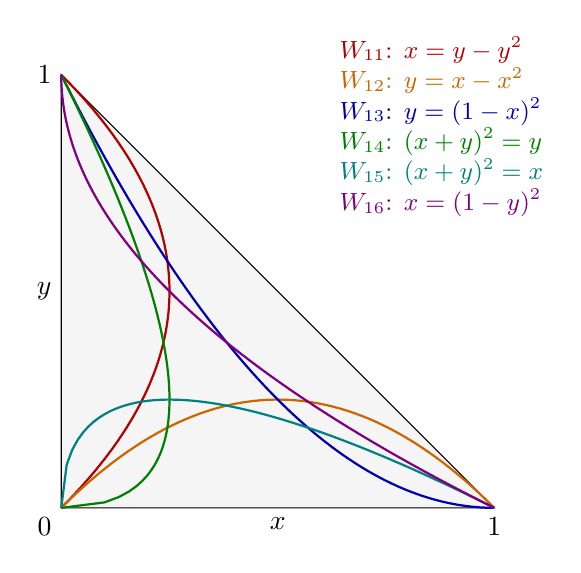
\begin{tikzpicture}[scale=5.5]
  \fill[gray!8] (0,0)--(1,0)--(0,1)--cycle; \draw (0,0)--(1,0)--(0,1)--cycle;
  \node[below left] at (0,0) {$0$}; \node[below] at (1,0) {$1$}; \node[left] at (0,1) {$1$};
  \node[below] at (0.5,0) {$x$}; \node[left] at (0,0.5) {$y$};
  \draw[thick,red!70!black,domain=0:1,samples=60,variable=\t] plot ({\t-\t*\t},\t);
  \draw[thick,orange!80!black,domain=0:1,samples=60,variable=\t] plot (\t,{\t-\t*\t});
  \draw[thick,blue!70!black,domain=0:1,samples=60,variable=\t] plot (\t,{(1-\t)^2});
  \draw[thick,green!50!black,domain=0:1,samples=80,variable=\t] plot ({sqrt(\t)-\t},\t);
  \draw[thick,teal,domain=0:1,samples=80,variable=\t] plot (\t,{sqrt(\t)-\t});
  \draw[thick,violet,domain=0:1,samples=60,variable=\t] plot ({(1-\t)^2},\t);
  \node[font=\small,align=left,anchor=west] at (0.62,0.88) {
    {\color{red!70!black}$W_{11}$: $x=y-y^2$}\\ {\color{orange!80!black}$W_{12}$: $y=x-x^2$}\\
    {\color{blue!70!black}$W_{13}$: $y=(1-x)^2$}\\ {\color{green!50!black}$W_{14}$: $(x+y)^2=y$}\\
    {\color{teal}$W_{15}$: $(x+y)^2=x$}\\ {\color{violet}$W_{16}$: $x=(1-y)^2$}};
\end{tikzpicture}
\end{center}
\noindent Figure 3. The spurious curves of the quadratic letters in the decay triangle. Each runs into two corners.

%=====================================================================================================================
\part*{Part 4. Checks and precision}

\section{Leading colour against the exact GPL results}
The planar ($N_c^3$, $N_c^2N_f$, $N_cN_f^2$) parts of the remainders are known exactly in terms of GPLs (2024 planar
ancillary files).
\begin{center}\small
\begin{tabular}{lll}\toprule
check & points & result \\ \midrule
decay, $N_c^3$ vs \texttt{decay.m}, double & 406 grid points & median $10^{-13}$, worst $7\cdot10^{-10}$ \\
decay, $N_c^3$ vs \texttt{decay.m}, quad & 3 points & $3\cdot10^{-16}$ (reference precision) \\
region $y$, planar layers vs \texttt{lmL.m}, \texttt{lpL.m} & $3\times6\times3$ values & worst $1.5\cdot10^{-11}$ \\
\bottomrule
\end{tabular}
\end{center}
The published values are evaluated with GiNaC at 25 digits.
Region $y$ is the channel of the published production results, so this test also checks the analytic continuation
and the branch of the root against an independent computation.

\paragraph{Further checks, all colour layers.}
\begin{itemize}
\item In each region at one point, all 84 values, real and imaginary parts separately. The region evaluator agrees
  with a direct quad integration from the decay to $10^{-28}$--$5\cdot10^{-23}$. It agrees with the independent
  continuation through the corner (double) to $10^{-13}$--$2\cdot10^{-8}$, the accuracy of that method. Every layer
  has a sizeable imaginary part.
\item Double against quad at random points of the decay triangle, all 84 values: median actual error $2\cdot10^{-12}$
  in the bulk.
\end{itemize}

\section{Precision on the LHC phase space}
\paragraph{The domain.} In a production region (e.g.\ $z>1$) with jet energy $E_j$ and angle $\theta$ in the partonic
frame, $u=E_j(1+\cos\theta)/\sqrt{\hat s}$ and $w=E_j(1-\cos\theta)/\sqrt{\hat s}$, so
\[
  \frac{p_T^2}{M_Z^2}=\frac{u\,w}v,\qquad \frac uw=e^{2\eta^*},\qquad\sqrt{\hat s}=\frac{M_Z}{\sqrt v}.
\]
Threshold ($v\to1$) and the collinear edges ($u,w\to0$) have $p_T\to0$. We take
$15\,\text{GeV}<p_T<2\,\text{TeV}$, $\sqrt{\hat s}\le13.6$ TeV (the collider energy) and the jet acceptance
$|\eta^*|\le4.5$. In $(u,v)$, with $\kappa_1=(15/91.19)^2=0.0271$ and $\kappa_2=(2000/91.19)^2=481$, this is
\[
  \kappa_1v\le u\,w\le\kappa_2v,\qquad v\ge4.5\cdot10^{-5},\qquad e^{-9}\le u/w\le e^9 .
\]
It implies $v\le0.72$ and $u,w\ge1.2\cdot10^{-4}$.

\begin{center}
\newcommand{\ptpanel}[4]{%
\begin{tikzpicture}[scale=3.9]
  \fill[gray!8] (0,0)--(1,0)--(0,1)--cycle; \draw (0,0)--(1,0)--(0,1)--cycle;
  \fill[#4!30,domain=0.00005:#2,samples=150,variable=\v]
     plot ({((1-\v)-sqrt(max((1-\v)^2-4*#1*\v,0)))/2},\v) --
     plot[domain=#2:0.00005] ({((1-\v)+sqrt(max((1-\v)^2-4*#1*\v,0)))/2},\v) -- cycle;
  \draw[#4!70!black,thick,domain=0.00005:#2,samples=150,variable=\v]
     plot ({((1-\v)-sqrt(max((1-\v)^2-4*#1*\v,0)))/2},\v);
  \draw[#4!70!black,thick,domain=0.00005:#2,samples=150,variable=\v]
     plot ({((1-\v)+sqrt(max((1-\v)^2-4*#1*\v,0)))/2},\v);
  \draw[dashed,gray] (0,#2) -- (1-#2,#2);
  \node[left,font=\scriptsize] at (0,#2) {$#2$};
  \node[below,font=\small] at (0.5,0) {$u$}; \node[left,font=\small] at (0,0.22) {$v$};
  \node[below left,font=\scriptsize] at (0,0) {$0$}; \node[below,font=\scriptsize] at (1,0) {$1$};
  \node[left,font=\scriptsize] at (0,1) {$1$};
  \node[font=\small,align=left,anchor=west] at (0.38,0.86) {$p_T>#3$ GeV\\ $\kappa_1=#1$};
\end{tikzpicture}}%
\ptpanel{0.0271}{0.72}{15}{blue}\hspace{4mm}%
\ptpanel{0.0752}{0.58}{25}{teal}\hspace{4mm}%
\ptpanel{0.1473}{0.47}{35}{orange}
\end{center}
\noindent Figure 4. The domain $u\,w\ge\kappa_1v$ for $p_{T,\min}=15$, 25 and 35 GeV; the largest $v$ is dashed. The
energy and rapidity cuts act at the $10^{-4}$ scale near the corners, where they cannot be seen on this scale.

\paragraph{The test} (\texttt{accuracy\_study/pheno\_domain\_check.py}).
\begin{itemize}
\item \textbf{Points:} about 330 per region, log-spaced in $v$ and dense towards both collinear edges.
\item \textbf{Double:} every point, with its estimate (method 2).
\item \textbf{Quad:} the three worst points (by estimate) of each band of $\min(u,w)$ in each region, giving the actual
  error (method 1).
\item \textbf{Values:} all 84, i.e.\ all six helicity coefficients and all colour layers. We quote the colour-summed
  coefficients ($N_c=3$, $N_f=5$, $N_{f,Z}=1$, the worst of the six) through the bound
  $\sum_l|c_l|\,|\delta_l|/|\sum_lc_la_l|$.
\end{itemize}

\paragraph{Results.} Error of the colour-summed coefficients in double, at the checked points of all three regions:
\begin{center}
\begin{tabular}{lll}\toprule
$\min(u,w)$ & without the rapidity cut & with $|\eta^*|\le4.5$ \\ \midrule
$\ge10^{-3}$ & $10^{-8}$ -- $6\cdot10^{-6}$ & median $1.2\cdot10^{-6}$, worst $3.4\cdot10^{-6}$ \\
$10^{-4}$ -- $10^{-3}$ & $4\cdot10^{-7}$ -- $9\cdot10^{-6}$ & median $1.1\cdot10^{-6}$, worst $8.7\cdot10^{-6}$ \\
$2\cdot10^{-5}$ -- $10^{-4}$ & $3\cdot10^{-5}$ -- $10^{-4}$ & outside the domain \\
$<2\cdot10^{-5}$ & $10^{-3}$ -- $O(1)$ & outside the domain \\ \bottomrule
\end{tabular}
\end{center}
\begin{itemize}
\item \textbf{The failing corner.} Without a rapidity cut, the failing points are jets with $\sqrt{\hat s}\gtrsim100\,p_T$
  ($\eta^*\gtrsim4.6$), outside the detector acceptance.
\item \textbf{Individual layers.} Some single colour layers have large relative errors where they are $10^4$--$10^6$
  times smaller than the others. Relative to the largest value at the point the error is at most $4\cdot10^{-6}$.
\end{itemize}

\paragraph{Conclusion.} On the LHC domain the double evaluator gives the colour-summed coefficients to better than
$10^{-5}$ in all three regions, typically $10^{-6}$. The worst points are at the forward edge of the acceptance and at
the highest $p_T$ and energy. A strict $10^{-6}$ everywhere needs quad at those points. The statement rests on the
points checked in quad. Running quad at every point whose estimate exceeds $10^{-6}$ (1--2 hours) would make it
airtight.

%=====================================================================================================================
\appendix
\section*{Appendix: where things are}
\begin{center}\footnotesize
\begin{tabular}{ll}\toprule
\texttt{iter int /generators\_deq/iisys.py} & closure, orthonormal system \\
\texttt{integral\_basis.py}, \texttt{out/basis.wl}, \texttt{out/deq.wl} & integer system (586 functions) \\
\texttt{quad\_data.py} & double series and chart series at the corners; quad runs \\
\texttt{cpp/tridents\_bs.cpp}, \texttt{cpp/iter\_quad.cpp} & integrators: double, double-double \\
\texttt{quad\_p0\_to\_double.py} & exact map from the 586 functions $F$ to the states $\phi_n$ \\
\texttt{region\_p0.py}, \texttt{region\_quad.py} & region $P_0$ from the series; direct transport (cross-check) \\
\texttt{gen\_eval.py}, \texttt{remainder\_eval.py} & double evaluation, path choice, spurious averaging, estimate \\
\texttt{quad\_eval.py}, \texttt{remainder\_quad.py}, \texttt{ddnp.py} & quad evaluation \\
\texttt{region\_lc\_check.py}, \texttt{region\_continuation\_check.py} & checks against published results; continuation \\
\texttt{accuracy\_study/pheno\_domain\_check.py} & precision on the LHC domain \\
\texttt{package/} & the shippable package \texttt{zgqq\_eval} \\ \bottomrule
\end{tabular}
\end{center}

\end{document}
